\section*{Implementation}
To prove the same method contract expressed as pre/post-condition, it is easier to use recursive approach compared to iterative approach (which involves loops and loop invariant). It is natural for humans to think about questions in top-down manner and solve them via divide and conquer; as a result, it is easier to come up with the recursive functions that persuade Dafny that the method contracts have been satisfied by the implementation. However, the project is required to develop Dafny code that use loop invariant, therefore, only the iterative approach will be discussed here.

\bigskip
In this section, the implementation and proof of delete method (which is the most complex one) will be exemplified. The other methods were implemented and proved in a similar way and will be skipped here.\\

The implementation of method delete(index:int) is divided into two classes: INode and INodes respectively. This is for the convenience of handling the situation where the last node is deleted from the list. There is a dummy node in the INodes that never gets deleted, storing no list data but pointing to the first real node in the list.

\subsection*{Fields and ghost fields of class INode}
\begin{lstlisting}
ghost var tailContents: seq<Data>;
ghost var spine: seq<INode>;
ghost var footprint: set<INode>;

var data: Data;
var next: INode;
\end{lstlisting}

There are two fields in a linked-list node: data and next, where the data can be of any type, and next is of type INode which denotes the next node referenced by the current node.\\

The three ghost variables, namely tailContents, spine and footprint, represent the data sequence starting from the next node, the whole list in sequence form, and the reachable nodes from the current node, respectively.

\subsection*{class invariant for INode}
\begin{lstlisting}
predicate good()
reads this, footprint;
{
    this in footprint 
	&& (next != null ==> (next in footprint 
	&& this !in next.footprint 
	&& footprint == {this} + next.footprint
	&& spine == [this] + next.spine
	&& tailContents == [next.data] + next.tailContents
	))
	&& (next ==null ==> tailContents == [] && footprint == {this}
				&& spine == [this])
}

predicate Valid()
reads this, footprint;
{
good()  
&& (next != null ==> next.Valid())
}
\end{lstlisting}  

The predicate $Valid()$ in the above code defines the class invariant of a linked-list node. It describes the structural property of the linked list, for both the singleton list and list with more than one nodes. This property is held since the object of the INode is created by the constructor, and will be maintained by all the operations performed on the object.

\begin{figure}[htbp]
\centering
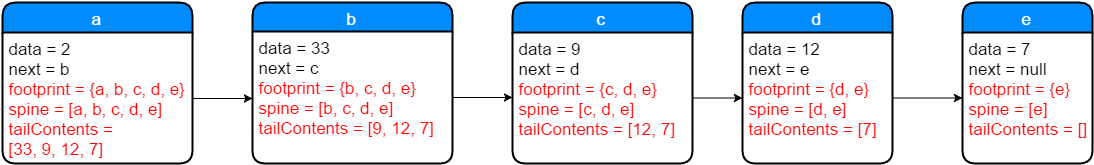
\includegraphics[width=0.81\textwidth]{./Diagrams/ValidLinkedList}
\caption{The graph notation of a valid linked-list}
\label{fig:ValidLinkedList}
\end{figure}

\subsection*{A heavily used lemma}

\begin{lstlisting}
predicate ValidLemma()
requires Valid();
reads this, footprint;
ensures ValidLemma();
ensures (forall nd :: nd in spine ==> nd in footprint);
ensures |tailContents| == |footprint|-1 == |spine|-1;
ensures forall nd :: nd in spine ==> nd != null && nd.Valid();
ensures forall nd :: nd in footprint ==> nd != null && nd.Valid();
{
if next == null then (spine == [this])
else (
spine == [this] + next.spine 
&& next.ValidLemma())
}

\end{lstlisting}

The ValidLemma() summarizes some valid consequence of the Valid() property which helps the procedure of proving complex properties. 

\begin{lstlisting}
	method delete(pos:int) returns (delNd:INode)
	requires Valid();
	requires 0 < pos <= |tailContents|;
	
	modifies footprint;
	
	ensures Valid();
	ensures [data] + tailContents == old(([data] + tailContents)[0..pos] + ([data] + tailContents)[pos+1..] );
	ensures footprint == old(footprint) - {delNd};
	
	{
	var curNd := this;
	var curIndex := 0;
	
	assert ValidLemma();
	assert ndValid2ListValidLemma();
	assert validSeqContentsLemma();
	assert validSeqTCLemma(spine);
	
	while (curIndex < pos-1)
	invariant 0 <= curIndex < pos;
	invariant curNd != null && curNd.Valid();
	invariant validSeqCond(spine);
	invariant |curNd.tailContents| + curIndex == |tailContents|;
	invariant curNd.next != null;
	invariant curNd == spine[curIndex];
	
	invariant  spine[curIndex].data == ([data] + tailContents)[curIndex];
	
	invariant curNd.next == spine[curIndex+1];
	invariant curNd.next.next != null ==> curNd.next.next == spine[curIndex+2];
	
	modifies {};
	{
	curNd := curNd.next;
	curIndex := curIndex + 1;
	}
	
	delNd := curNd.next;
	
	delNext(curNd, delNd, pos);
	
	
	if(1 < pos <= |tailContents|) {
	ghost var oldContents := old([data] + tailContents); 
	ghost var newSpine := spine[0..pos-1];
	
	assert delNd != null;
	
	updateSeq4Del(newSpine, delNd, pos, curNd, oldContents, this);
	
	} else {}
	
	}
\end{lstlisting}

To present the structure of proof more clearly, the operation of delete is divided into three parts: the first part contains a loop that iterating the list and stops at the node whose next one is the node that is going to be deleted. Then the deletion is achieved by the second part, which is an invocation of the method delNext(curNd:INode, delNd:INode, pos:int); Finally, the ghost variables are updated in the ghost method 'updateSeq4Del'; This layout gives a clearer structure and also enables me to specify accurate frame conditions neatly for each sub-operation.

\bigskip

The code to prove the delete(index:int) operation used several predicates, some of them specify the properties held by different portions of the list at certain program points; others specify the properties held by the whole list, but with different strength, which reflect the properties held by the whole list at different phases. Certain predicates are not directly clear but can be deduced by providing proper lemmas. In the next section, several predicates used in the code will be exemplified.

\subsection*{Some Predicates}
\begin{lstlisting}[caption=valid sequence predicate]
predicate validSeqCond(mySeq: seq<INode>)
reads mySeq, (set nd | nd in mySeq);
{
listCond(mySeq) 
&& (mySeq != [] ==> mySeq[|mySeq|-1].next == null
&& mySeq[|mySeq|-1].footprint == {mySeq[|mySeq|-1]}
&& mySeq[|mySeq|-1].tailContents == []
&& mySeq[|mySeq|-1].spine == [mySeq[|mySeq|-1]])
}
\end{lstlisting}

The predicate of valid sequence defines the property of a valid sequence which is isomorphic to a linked-list. So, given a valid linked-list node, its ghost field 'spine' must satisfy the validSeqCond property. And vice versa, given a valid sequence, the first node of the sequence must be valid and its spine field must be equal to the whole sequence.

\bigskip
When some node in the list is updated, it will break the properties of all the nodes from which the changed node can be reached, while the next node linked by the changed node will not be affected. For example, the 'i'th node in a list is updated, then it will immediately invalidate all the nodes with indices less than or equal to i, however, all the nodes with indices that are large than i will not be affected.

\bigskip
Even though the stronger property 'validSeqCond' may not hold after a change in the member node, some weaker properties of the list may still hold, like the property 'listInv'\\

\begin{lstlisting}[caption=list invariant property]
predicate listInv(mySeq: seq<INode>)
reads mySeq, (set nd | nd in mySeq);
{
null !in mySeq && (forall nd :: nd in mySeq ==> nd in nd.footprint) &&
(forall i :: 0 <= i < |mySeq|-1 ==> mySeq[i].next == mySeq[i+1])
&& (forall i, j :: 0 <= i < j < |mySeq| ==> mySeq[i] !in mySeq[j].footprint)
}
\end{lstlisting}

\bigskip
In the case where the $i$th node is deleted, then the No.$i-1$ node's next field will be set to point to No.$i+1$ (if there is any) (we require the first node should not be deleted in INode class). Because nothing in the subsequence of $spine[0..i]$, say $s_1$, is changed except the next field of the last element in $s_1$, so the following $listCond$ property is held on the sequence $s_1$. 

\begin{lstlisting}
predicate listCond(mySeq: seq<INode>)
reads mySeq, (set nd | nd in mySeq);
{
null !in mySeq && (forall nd :: nd in mySeq ==> nd in nd.footprint) &&
(forall i :: 0 <= i < |mySeq|-1 ==> mySeq[i].next == mySeq[i+1]
&& mySeq[i].footprint == {mySeq[i]} + mySeq[i+1].footprint
&& mySeq[i].tailContents == [mySeq[i+1].data] + mySeq[i+1].tailContents
&& mySeq[i].spine == [mySeq[i]] + mySeq[i+1].spine)
&& (forall i, j :: 0 <= i < j < |mySeq| ==> mySeq[i] !in mySeq[j].footprint)
}
\end{lstlisting}

\bigskip

Another segment of the spine field, say $s_2 = spine[i+1..]$, is the same as before, so it is still a valid sequence which satisfies $validSeqCond$ property.\\

Therefore, to make the all the nodes in the list become valid again, we only need to update the ghost fields in sequence $s_1$ so that the ghost fields reflect the real data structures. In the sequence $s_1$, we also observes that $s_1[i+1]$ is valid if $i+1$ is a valid index of the sequence $s_1$.

\bigskip

So at this moment, we actually have already found the loop invariant which enables us to prove the Valid() property after updating the nodes in the sequence $s_1$. We did the proof inside the following separate ghost method called $updateSeq4Del$\\

\begin{lstlisting}
ghost method updateSeq4Del(newSpine: seq<INode>, delNd:INode, pos: int, nxtNd:INode, oldContents:seq<Data>, thisNd:INode)
\end{lstlisting}


The above code snippet is inside a separate method which is dedicated for updating the ghost variables, and when it is invoked, the caller will send $old([data] + tailContents)$ as argument for the parameter $oldContents$, which reflects the content of the list before performing the delete operation.\\


To perform the iterative updates, we need to traverse the nodes in the sequence from right to left; and in the loop body, we need to update the footprint, tailContents and spine field of the node at that iteration (i.e. node with index $i$) so that the node $s_1[i]$ visited at that iteration becomes valid again. Then we decrement the index i so that 
the loop invariant holds again: $s_1[0..i]$ and  $s_1[i+1..]$ satisfies the  $listCond$ property, and $s_1[i+1]$ is valid.\\

At the end, when we exit the loop, index i becomes -1 and therefore the first node $s_1[0]$ in this sequence, which is the node upon which we performed the delete operation, is valid.

\bigskip

However, we should not stop here; it is easy to provide an implementation that makes the current node valid after the operation, we can in fact delete everything except the first node and still makes the node valid; but that's not desirable.
Therefore, we need to ensure another post condition: $[data] + tailContents == old(([data] + tailContents)[0..pos] + ([data] + tailContents)[pos+1..] );$ through which we can guarantee that we only delete the data at the specified position.\\

We proved that post condition by adding the following loop invariant into the loop's annotation block:\\

$invariant -1 <= curIndex < pos - 2 ==>  [newSpine[curIndex+1].data] + newSpine[curIndex+1].tailContents == oldContents[curIndex+1..pos] + oldContents[pos+1..];$\\

$	invariant thisNd == newSpine[0];$\\

When we exit the loop, curIndex becomes -1 and we can get the desired post condition about list contents successfully.

\subsection*{Implementation Style}
During the implementation, besides the traditional method invocation and while loops, I also tried something similar to the \emph{Basic Path} approach for generating the verification condition. Basically, I identified different parts of the method which are separated by pre/post conditions and loop invariants, and implemented the following methods/predicates:\\

\begin{itemize}
\item LI: predicate for expressing loop invariant.
\item pre2LI: which is a method that verifies executing the initialization code at the state which satisfies the pre-condition will result in a state which satisfies the loop invariant.

\item LIGuardExecBody2LI: Executing the loop body in a state which satisfies the loop invariant and loop guard will result in a state that still satisfies the loop invariant.

\item LIAndNegGuard2Post: it is in fact a lemma that checks the fact that loop invariant together with the negation of the loop guard will imply the post condition.
\end{itemize}
